\documentclass[a4paper, 12pt]{article}
\usepackage{barinov}
\begin{document}
\thispagestyle{empty}
\begin{center}
    \textit{Федеральное государственное автономное образовательное\\ учреждение высшего образования }

    \vspace{0.5ex}

        \textbf{«Московский физико-технический институт\\ (национальный исследовательский университет)»}
\end{center}

\vspace{10ex}

\begin{center}
    \vspace{13ex}

    \so{\textbf{Лабораторная работа №-.-.-}}

    \vspace{1ex}

    по курсу общей физики

    на тему:

    \textbf{\textit{<<>>}}

    \vspace{30ex}

    \begin{flushright}
        \noindent
        \textit{Работу выполнил:}\\  
        \textit{Баринов Леонид \\(группа Б02-827)}
    \end{flushright}
    \vfill
    Долгопрудный \\2019
\newpage
\setcounter{page}{1}
\fancyhead[R]{\nouppercase{\leftmark}}	
\end{center}

\section{Аннотация}
В работе будут исследованы методы получения анализа поляризованного
света.






\section{Теоретические сведения}
\subsection*{Получение эллиптически поляризованного света}
Эллиптически поляризованной свет можно получить из линейно
поляризованного с помощью двоякопреломляющих кристаллических
пластинок.

\begin{wrapfigure}{r}{0.3\linewidth}
    \includegraphics[width=\linewidth]{1}
    \caption{Разложение линейно поляризованного света по главным
    направлениям двоякопреломляющей пластинки}
    \label{fig:1}
\end{wrapfigure}

Двоякопреломляющая пластинка имеет два взаимно перпендикулярных
главных направления, совпадающих с осями эллипсоида диэлектрической
проницаемости. Волны, поляризованные вдоль главных направлений,
распространяются в пластинке с разными скоростями, не изменяя
характера своей поляризации. Эти волны называются главными. Мы будем
обозначать показатели преломления для главных волн через $n_x$ и
$n_y$, где $x$ и $y$ --- главные направления кристаллической пластинки
\fig{fig:1}.

Пусть на пластинку падает линейно поляризованная волна, электрический
вектор которой ориентирован под некоторым углом $\alpha$ к оси $x$.
Разложим вектор $\vv{E}$ на составляющие $E_x$ и $E_y$. На входе
пластинки $E_x$ и $E_y$ находятся в фазе. На выходе из-за разности
скоростей между ними появляется разность хода $d(n_x-n_y)$, при этом
сдвиг фаз определяется соотношением:
\begin{equation}
    \Delta \phi = \frac{2\pi}{m}= kd(n_x-n_y)
    \label{eq:1}
\end{equation}
где $k$ --- волновое число (в пустоте), $d$ --- толщина
кристаллической пластинки.

Рассмотрим практически важные частные случаи

\begin{wrapfigure}[13]{l}{0.3\linewidth}
    \includegraphics[width=\linewidth]{2}
    \caption{Поворот направления колебаний с помощью пластинки в
    $\lambda/2$}
    \label{fig:2}
\end{wrapfigure}

Пластинка дает сдвиг фаз $2\pi$ (пластинка в длину волны $\lambda$). В
результате сложения волн на выходе пластинки образуется линейно
поляризованная волна с тем же направлением колебаний, что и в падающей
волне.

Пластинка дает сдвиг фаз $\pi$ (пластинка в полдлины волны
$\lambda/2$). На выходе пластинки снова образуется линейно
поляризованная волна. Направление $bb'$ колебаний этой волны повернуто
относительно направления $aa'$ колебаний падающей волны (\fig{fig:2}).
Направление $bb'$ является зеркальным отображением направления $aa'$
относительно одного из главных направлений пластинки. Такую пластинку
используют для поворота направления колебаний линейно поляризованного
света.

Пластинка создает между колебаниями сдвиг фаз $\pi/2$ (пластинка в
четверть длины волны). При сложении двух взаимно перпендикулярных
колебаний, имеющих разность фаз $\pi/2$, образуется эллипс, главные
оси которого совпадают с координатными осями $x$ и $y$. При равенстве
амплитуд $E_x^\text{max} = E_y^\text{max}$ возникает круговая
поляризация.

\subsection*{Пластинка чувствительного оттенка}

\begin{wrapfigure}{l}{0.25\linewidth}
    \includegraphics[width=\linewidth]{3}
    \caption{Пластинка чувствительного оттенка}
    \label{fig:3}
\end{wrapfigure}

Пластинка имеет форму стрелы (\fig{fig:3}), вдоль оси которой
расположено главное направление, соответствующее большей скорости
распространения.

Если между скрещенными поляроидами поместить пластинку чувствительного
оттенка ($\lambda$) и пластинку $\lambda/4$ так, чтобы их главные
направления совпадали, цвет пластинки изменится. Если у пластинки
чувствительного оттенка и пластинки в $\lambda/4$ совпадут главные
направления, соответствующие большей скорости распространения, то
разность хода между $E_x$ и $E_y$ для зеленого света составит уже
$5\lambda/4$. Это соответствует разности хода в $\lambda$ для света с
большей длиной волны.


\section{Оборудование}







\section{Результаты измерений и обработка результатов}







\section{Обсуждение результатов и выводы}







\end{document}
